\chapter{Välkommen till Vintergatan}

När vi tittar upp mot himlen en mörk, stjärnklar natt, så kan vi se ett 
ljusstarkt band sträcka sig över himlen. Om du tittar med en kikare eller
med ett teleskop, som Galileo gjorde år 1609, så upptäcker du att bandet
består av ett stort antal stjärnor. Detta är vår galax, {\bf Vintergatan},
så som den ser ut från jorden. Den består av omkring hundra miljarder
stjärnor, och Solen är en av dem. Det finns många andra galaxer i Universum.

Det tog lång tid för astronomer att förstå hur Vintergatan verkligen ser ut.
Man skulle vilja åka ut i ett rymdskepp och observera galaxen utifrån, men det
kommer aldrig att kunna gå eftersom den resan är för lång.  Vi måste därför
bestämma Vintergatans struktur från vår egen plats inuti den. 

Observationer med optiska- och radioteleskop av Vintergatan och andra galaxer
har använts för att förstå Vintergatans struktur. Idag så har vi mycket kunskap
om vår galax; den består av en skiva (disk) av stjärnor och gas, som är
fördelade i olika spiralarmar.

När man äntligen trodde att man förstod hur Vintergatan var uppbyggd, uppkom
ett nytt mysterium! Man observerade hastigheterna hos stjärnor långt ut i
galaxen, och kunde se att de roterade alldeles för snabbt i förhållande till
hur mycket massa man kunde se. Man tror nu att galaxen innehåller stora mängder
av {\bf mörk materia}, något som vi inte kan se men som påverkar galaxens
rörelse genom gravitation. Man kan jämföra den mörka materiens inverkan med en
man och en kvinna som dansar i ett helt mörkt rum. Mannen har på sig mörka
kläder och syns därför inte, medan kvinnan har på sig självlysande färger. När
de dansar, ser man bara kvinnan, inte mannen, men man förstår att mannen måste
vara där eftersom annars skulle kvinnan flyga iväg då hon har väldigt hög fart.
Radioobservationer har hjälpt till att upptäcka den mörka materian, men man vet
fortfarande inte vad den består av.

\vfill\eject
\section{Vår plats i Vintergatan}
Vår stjärna, Solen, och dess solsystem, befinner sig i den yttre delen av
Vintergatan, ungefär 8,5 kpc\footnote{1 kpc = 1 kiloparsec = 10$^3$ pc; 1
parallax-sekund (parsec, pc) = 3.086$\cdot 10^{16}$~m.}  (25000 ly\footnote{1
ljusår (ly) = 9.4605$\cdot 10^{15}$~m}) från galaxens centrum. Den största
delen av gasen och stjärnorna finns i den tunna skiva och roterar runt galaxens
centrum. Solen roterar runt centrum av galaxen med en hastighet av 220 km/s och
tar ca 240 miljoner år på sig att fullfölja ett varv runt galaxen.

\section{Galaktiska koordinater: longitud och latitud}
\label{sect:galcoords}
För att beskriva positioner för astronomiska objekt använder man olika
typer av koordinatsystem. I vår galax är det smidigt att använda det
galaktiska koordinatsystemet ($l,b$), där $l$ är den galaktiska
\emph{longituden} och $b$ är den galaktiska \emph{latituden} (se figur 
\ref{figdisc} och \ref{figmwsketch}). Koordinatsystemet är centrerat
kring solen. $b=0^{\circ}$ motsvarar riktningar i det galaktiska
planet. Latituden $b=90^{\circ}$ kallas den Galaktiska Nordpolen. Longituden
$l$ mäts moturs från riktningen från solen mot det galaktiska
centrumet, som alltså har koordinaterna $(l=0, b=0)$. I galaxens
centrum finns något väldigt speciellt; en stor massa som är ungefär
tre miljoner gånger tyngre än solen. Vi vet idag att det är ett
väldigt massivt svart hål. Från detta område, kallat Sagittarius A,
har astronomer detekterat stark radio- och röntgenstrålning.

\begin{figure}[ht]
\begin{center}
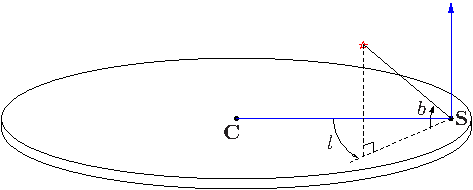
\includegraphics[width=8cm]{../figures/galdisc.pdf}
\end{center}
\caption{Illustration av det galaktiska koordinatsystemet, med longitud ($l$)
och latitud ($b$).  {\bf C} makerar det galaktiska centret, {\bf S} solen.}
\label{figdisc}
\end{figure} 

\begin{figure}[ht]
\begin{center}
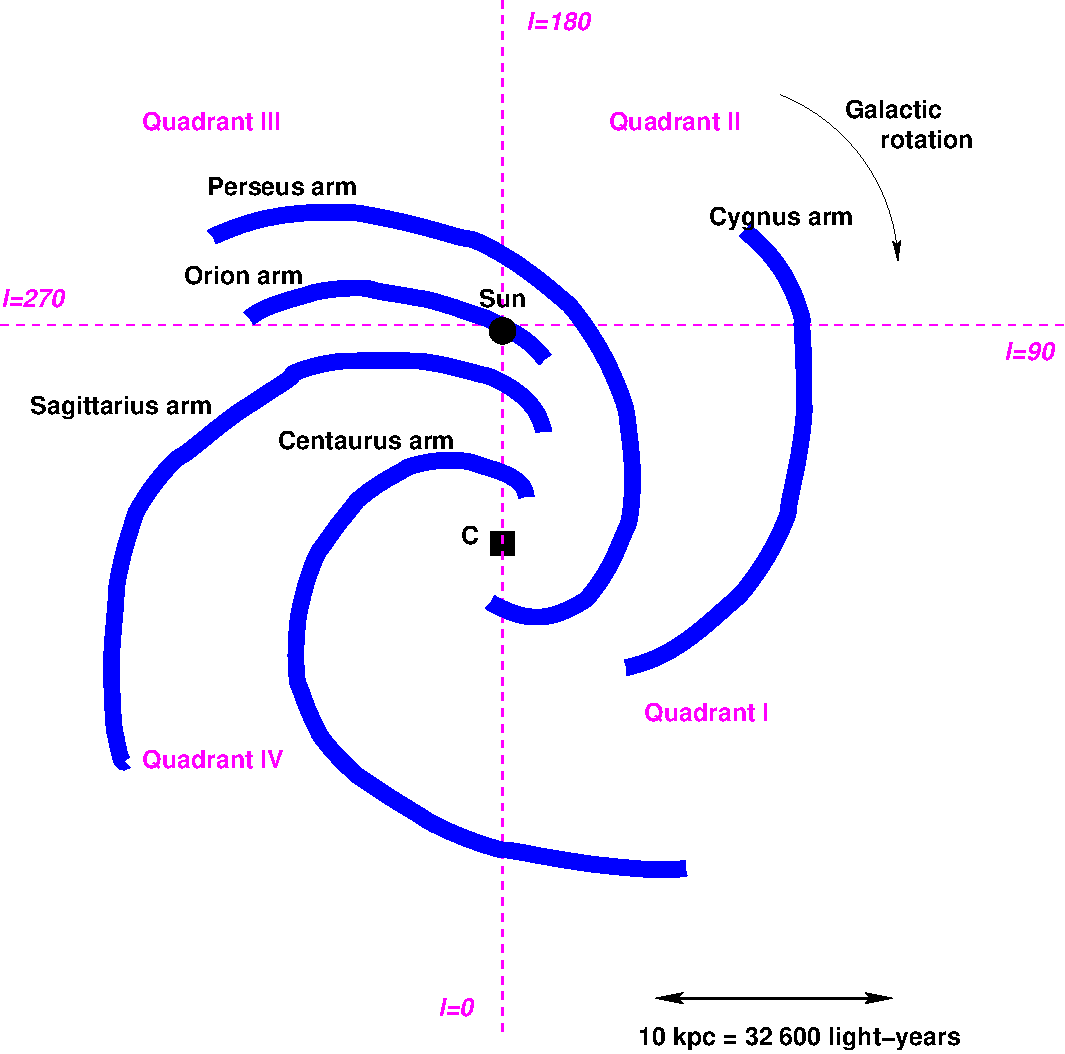
\includegraphics[width=10cm]{../figures/mwsketch.pdf}
\end{center}
\caption{ En skiss över Vintergatans spiralstruktur. Galaxens centrum är vid
punkten {\bf C}. De fyra kvadranterna är markerade som Quadrant I till IV. }
\label{figmwsketch}
\end{figure}  

Galaxen kan delas in i fyra kvadranter betecknade med Romerska tal: 
\bigskip
\begin{displaymath}
\begin{array}{lc}
\hbox{Kvadrant {\sc I}} 	&0\deg < l < 90\deg	\\
\hbox{Kvadrant ${\rm II}$} 	&90\deg < l < 180\deg	\\
\hbox{Kvadrant ${\rm III}$} 	&180\deg < l < 270\deg	\\
\hbox{Kvadrant ${\rm IV}$} 	&270\deg < l < 360\deg 
\end{array}
\end{displaymath}
\bigskip

I första och fjärde kvadranten så observerar vi framförallt den inre delen
av vår galax. Kvadranterna tre och fyra innehåller materia som är längre
bort från galaxens centrum än Solen. 

\section{Radiovågor från atomärt väte}
Den största delen av gasen i Vintergatan är i form av atomärt väte (H).  Väte
är den enklaste atomen, den har bara en proton och en elektron.  Atomärt väte
skickar ut radiovågor med våglängden $\lambda= 21$~cm (eller en frekvens
på$f=c/\lambda=1420$~MHz, där $c\simeq 300 000\, {\rm km/s}$ är ljusets
hastighet). Det är denna signal som vi vill mäta med SALSA.

\begin{equation}
\boxed{
\lambda = 21 \, {\rm cm}
\Rightarrow f=c/\lambda = 1420 \, {\rm MHz}}
\end{equation}

Vätelinjen uppkommer när elektronens spinn byter riktning från att vara
parallellt till anti-parallellt med protonens (se figur \ref{fighyperfin}).
Det resulterar i att atomen går ner till det lägre energitillståndet, (se
fig~\ref{fighyperfin}). Spinn är en kvantmekanisk egenskap hos partiklar som
enklast kan förklaras med att partikeln roterar kring sin egen axel. För
väteatomen kan man räkna ut att den totala energin är mindre då spinnen är
anti-parallella. Eftersom naturen alltid strävar mot att vara i ett så lågt
energitillstånd som möjligt, kommer väteatomer där spinnen är parallella att gå
över i det lägre energitillståndet med en viss sannolikhet. Övergången sker
spontant ungefär efter tio miljoner år för en väteatom, men eftersom det finns
så otroligt många väteatomer i universum blir vätelinjen väldigt stark. 

Den Holländske astronomen H.C. van de Hulst förutspådde teoretiskt att
21 cm linjen skulle finnas år 1945. Linjen detekterades för första
gången år 1951 av tre forskargrupper i USA, Holland och Australien (se
Appendix~\ref{app-history}).

\begin{figure}[ht]
\begin{center}
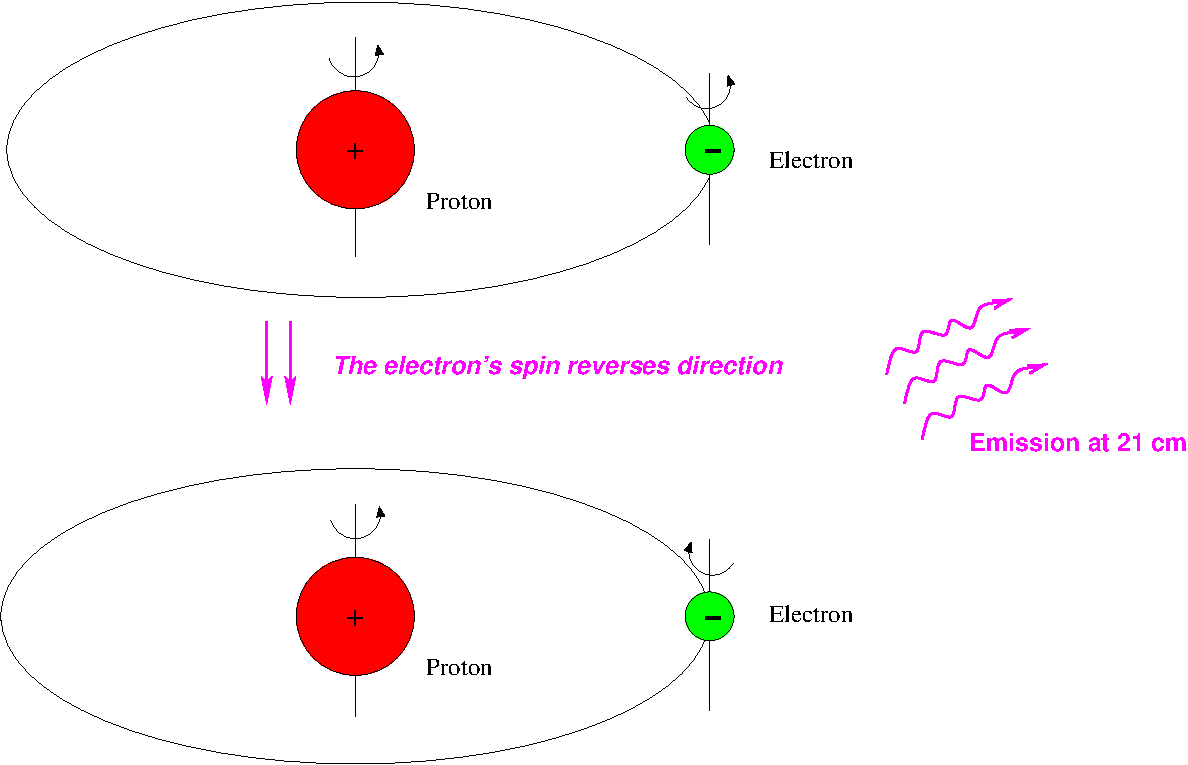
\includegraphics[width=10cm]{../figures/hyperfine.pdf}
\end{center}
\caption{Illustration av 21~cm övergången hos väteatomen, vilken orsakas
  av energiändringen då elektronens spinn ändras från parallellt till
  antiparallellt jämfört med protonens.}
\label{fighyperfin}
\end{figure}  

\section{Dopplereffekten}
Genom att observera radiovågor från väte så kan vi lära oss om rörelsen
för vätgasmolnen i Vintergatan. Det är nämligen möjligt att relatera den
observerade {\em frekvensen} till{\em hastigheten hos det strålande molnet}, 
genom den så kallade {\em Dopplereffekten}.

Denna effekt, uppkallad efter den österrikiske fysikern Christian Johann Doppler
(1803--1853), finns också i vår vardag; till exempel om du står still på gatan 
och en ambulans färdas {\em mot } dig. Då hör du ambulansens sirener med {\em en högre
frekvens (tonhöjd)} än om ambulansen varit parkerad på gatan. På samma sätt
så blir tonen lägre om ambulansen åker {\em från } dig. Eftersom
ljudvågor färdas genom genom luften för att nå dig så kan du tänka dig att
vågorna pressas samman när ambulansen rör sig mot dig. Därför blir våglängden
kortare och du hör en högre frekvens. Detta är dopplereffekten. 

Vi kan använda dopplereffekten för att relatera den frekvens som vi observerar till
hastigheten hos det strålande vätgasmolnet genom en matematisk formel:

\begin{equation}
{\boxed{
\frac{\Delta f}{f_0}=-\frac{v}{c}
}}
\end{equation}

där

\begin{displaymath}
\begin{array}{ll}
  \Delta f=f-f_0    &\hbox{frekvensskiftet}, 	\\
  f		    &\hbox{observerad frekvens} 	\\
  f_0		    &\hbox{vilofrekvens}	\\
  v		    &\hbox{hastighet, $> 0$ om objektet vi observerar
    rör sig bortåt}	\\
                    &\hbox{$< 0$ om det rör sig mot oss.}
\end{array}
\end{displaymath}

För att observera radiovågor från vätgas i Vintergatan så ställer vi in 
mottagaren i vårt radioteleskop att mäta på frekvenser nära vilofrekvensen 
för vätelinjen, d.v.s. den frekvens vi skulle se om det inte fanns någon relativ
rörelse. Moln med olika hastighet visar sig då vid olika frekvenser. Frekvensen
skiftas uppåt eller nedåt beroende på om gasen rör sig mot os eller från oss. 
